\chapter{Attachments}

\subsection{Heuristic evaluation results}

\begin{enumerate}
    \item \textbf{How are things categorized?}
    
\textbf{Group member:} 
The first thing that you see when going to finn.no is lots of elements that is categories. It is up to 14 different categories, and each of the elements is visualized with symbols, alongside with a category name. That is an good combination to help the user to choose the right category when they are going to look after stuff to buy. With only having symbols, it would lead up to misunderstanding, since some symbols can be too old for someone (as an old telephone for the young people), or people can have different interpretations about the symbolse. It is a good way to categorize. 

\textbf{Assignment provider:}
Things are categorized by primary type like “Eiendom”, “Bil”, “Torget” and then categories by sub category under the primary category. Some categories have rather deep category trees.

    \item \textbf{How does search work?}

\textbf{Group member:} 
The search is also something you find on the first site. In the search it have been placed a placeholder/label with a few examples to help the user to know how or what they can search for. 

When searching for example “TV”, you will get how many hits you get for each categories. This is a good thing, since if you know that you are searching for a “TV” as in a television, then you know that you need to choose the category where you can find television, and not the category about apartment. 

\textbf{Assignment provider:}
Search works very well. When in a category the search only searches in that category, which is a rather powerful feature of the system. On the main page however, search works on all items on the site.

    \item \textbf{How many things can you see on a page before switching?}

\textbf{Group member:} 
When you are looking on all the hits you got by searching television, you can see up to 51 elements before you can switch to the next site. The buy elements is organized like it is tree elements side by side, and then a new line with tree new elements. 

\textbf{Assignment provider:}
50 items in the electronics category.

    \item \textbf{Can you create your own user?}

\textbf{Group member:} 
Yes it is possible to create your own user on finn.no. In the upper right corner of the front page, it says “My FINN”. When clicking on that you will be taken to a page where you got the opportunity to logg inn or make a user. When clicking on “make a user” you will need to fill in email and password. 

\textbf{Assignment provider:}
Yes. It’s fairly simple, but you do have to verify with BankID to authenticate your account.

    \item \textbf{Is it easy to find contact information?}

\textbf{Group member:} 
To find contact information to FINN, you need to scroll down to the footer. It is written with small texts, and can for someone be hard to find at first. It should be placed on top or more visible so the user don't need to look for it. But on the other hand the FINN’s contact information is not the most important thing, it is to find the contact information to the one you are gonna buy a item from.

Without clicking the advertisement, the only information you get is where the item is and if the are a company or private seller. When you click on the advertisement you will on the right side get the name of the seller and right below it you will find a button you can click that give you opportunity to send a message/email to the seller. With other words it is easy to find.

\textbf{Assignment provider:}
Yes, it’s easy to find contact information for both Finn.no and individual sellers.
	
    \item \textbf{How does navigation work?}

\textbf{Group member:} 
When doing navigation on the main page you go through the most important things first. You start with search. After that you will navigate through all of the category that exist and then through some popular advertisement. At last you navigate through the footer where social media and contact information is. 

When you are inside of an advertisement you navigate first through the picture and information about the item. After that you going through contact information about the seller. It feel neat and orientated to navigate through FINN.

\textbf{Assignment provider:}
As Finn.no is a site for selling and buying stuff navigation primarily works on item category. As a sales site the navigation is pretty effective.

    \item \textbf{Can you store things you are interested in?}

\textbf{Group member:} 
FINN offers a element that let you store advertisement that you are interesting or want to get information about it if it has been updated or of it still for sale. Before clicking the advertisement you will see on the ad that its a heart symbol. When clicking that you will store it in your favorit. You can also add it to favorit when you have clicked on it, it will show a element below the picture that says “Add to favorit”

\textbf{Assignment provider:}
Yes. If you have an account, you just need to push the heart or “Legg til favoritt”.
	
    \item \textbf{What does the buy item contain?}

\textbf{Group member:} 
On the item it shows picture(s) of the product, follow by the title for the advertisement. For som product it also shows specific things and equipment and below that you will see the price for it. After that you can read the description about the product.

\textbf{Assignment provider:}
There are no “Buy item” button on the site. As the site is an action site you need to message the seller to be able to buy the item. Professional sellers that use Finn.no to showcase their products have a “Buy in online store” button where you can buy the items. To buy stuff from private sellers you need to send the seller a message and then buy the item directly.
\end{enumerate}

\textbf{Summary}

Since both of the evaluators is having two different expertise it was expected to get some different result of the evaluating. That is good for seeing more than one perspective of looking into FINN’s website. This is what that have been found by following the eight heuristics: 

\textbf{1.  How are things categorized?}
Things are categorized by primary type and then by sub category. They also use symbols/icons to represent the categories. 

\textbf{2.  How does search work?}
The search is placed good where it is very simple
to find it. When using it, it will in a category only searches in that category, which is a powerful feature of the system. On the main page it will search for all of the items. 

\textbf{3.  How many things can you see on a page before switching?}
50 element is possible to see. 

\textbf{4.  Can you create your own user?}
Yes it is possible and very simple. When creating a user one need to use BankID to authenticate your account.

\textbf{5.  Is it easy to find contact information?}
Yes, it is simple to find contact information for the seller, but a little tricky to find contact information for FINN. It has not been prioritized since it will be some of the last thing one will get by navigating through the main page. 

\textbf{6.  How does navigation work?}
The navigation go through the most important first, with that it means sals items and it works alright. 

\textbf{7.  Can you store things you are interested in?}
If one is having a account, then it is possible to store things of interest. It is a button that can be clicked on for storing. 

\textbf{8.  What does the buy item contain?}
It contain picture, title, description and other important information that needed before buying. For private sellers one need to take direct contact/message the seller to buy the item. For professional sellers it will be displayed a “Buy in online store” button.

\newpage
\subsection{Test plan for usability testing}
\begin{enumerate}
  \item \textbf{Purpose:} This is where you describe the purpose of what you will find with this usability test.
  \item \textbf{Problem statement:} Here you need to make some kind of list of problems that you want to be answered through the test.
  \item \textbf{User profile:} This is where you need to describe what kind of users that is supposed to take the test. What age are they? What background information do they have on what they will be testing? It is important to describe your user to see if that will affect the results of the test.
  \item \textbf{Methodology:} This is more of an concrete way to describe how the test should be carried out. Often it is four steps that should be followed. Those four steps are: 
  \begin{enumerate}
  \item \textbf{Participant greeting and background questionnaire:} This is where you can greet the participants and make them feel welcome. Do a background questionnaire and make sure that an anonymity agreement is signed.
  
  \item \textbf{Orientation:} The participant will get a short, verbal and scripted introduction and orientation about the test.
  The purpose of the test will be explained and what is expected from them as a participant. The participant will also be informed that they will be observed, videotaped or audio taped.
  
  \item \textbf{Performance test:} The performance test consist of a series of tasks and/or scenarios that the participant will be asked to do while being observed. The observer will write down any of the participants behavior, comment and any other unusual circumstances that might affect the result of the test.       
  
  \item \textbf{Participant debriefing:} After the test is done, it's time for a debriefing with the participant. It should follow these steps:
  
  - Filling out some kind of a brief performance questionnaire of the usability of the system. 
  
  - Let the participant give an overall comment of her or his performance of the test.
  
  - Let the participant tell about errors or problems that occurred during the test.
  
  \end{enumerate}
  \item \textbf{Task list:} This will contain a list of tasks that the monitor of the test want the participants to do. This is in order for the monitor to be able to test the things that he or she wants to test.
  
  \item \textbf{Test environment and equipment requirements:} This one need to describe the environment that the participant will be in. Is the environment quiet and calm or is it a lot of disturbance around that can disturb and affect the test result? That is important to document.
  
  Alongside with a description of the environment, it can be necessary to write down what kind of equipment that will be needed to complete the test. An example can be if there is a need for a pen, paper or maybe a phone. 
  
  \item \textbf{Test monitor role:} This is a description of what kind of role the test monitor will have during the test. Is the monitor going to be closed or open. By that it means will the monitor be closed as in the participant wont get any help if they ask, or if the monitor will be open where the monitor can answer questions and give some leads.
  
  It will need to be describe what the test monitor will be looking for. If the test is recorded, are the monitor still gonna write notes during the test, or is he or she just gonna look at the recording afterwards?  
  
  \item \textbf{Evaluation measure:} This is what kind of information or data that will be collected through the testing. It can be how long the participant use to complete the task, how many errors that occurs or other things that is needs to be collected.

  \item \textbf{Test report contents and presentation:} This is what the usability test consist of, and what the reader can find. It mainly consists of the test plan, the result and findings found in the test.
\end{enumerate}

\newpage
\section{Transcription of interview}

Transcription of interview

I1: Interviewer 1, A
I2: Interviewer 2, M
R: Respondent

R: ja klar

I2: OK, så dere har ikke noe system for inventar?

R: Nei vi har ikke noe system foreløpig for inventar, hverken manuelt eller digitalt

I2: ok

R:Og vi er vel flere støkkær hver for oss, som tar for oss hver vår del av inventaret

R: Og jeg er vel den som har mest samla oversikten

I1: OK, så dere er da, dere er fler som følger med

R: ja ja. Vi er flere som skal ha, være involvert i rommet her

R: eh men jeg er vel den eneste som har drivet noe særlig med MakerSpace fram til ganske nylig, så foreløpig er det jeg som kan 3D printere og laseren 

I1: Er du ansatt for å være på MakerSpace?

R: Eh, nei jeg er ansatt som formidler, men alle sammen har jo flere oppgaver

I2: Skal jeg skrive?
I1: ok

R: En av oppgavene mine blant andre er eh, å ha ansvar for det rommet her. 

I1: Ja

I2: Ja, så da har dere ansatte som egentlig deler, ikke nødvendigvis fordeler ansvar men har kontroll på det dere har da? 

R: Idielt sett, men jeg har ikke kontroll på alt som er i det rommet her. For i noen av skapene her så har vi utstyr som brukes til undervisning.  

I2: Dere har det og, ja ok.

R: Og i noen av skapene så har vi komponenter som er ment til MakerSpace eh, de skapene der borte for eksempel. Der har vi alt som tilhører 3D printere 
I1: Ja, umm Låser dere bort noe av utstyret? 

R: Vi låser rommet

I1: Dere låser altså selve rommet men ikke skapene?

R: ja, nei vi har  ikke noen lås på skapene

I1: Nei ok

R: Foreløpig, og det er fordi atte hittil så har vi ikke brukt rommet uten at noen av oss er tilstede. Eh og vi lurer litt på kossen vi skal få til det i det hele tatt fordi mye av rommet ligger inne i senteret. Så for å åpne rommet så må vi åpne senteret. Så hittil så har ikke rommet vært i bruk når ikke senteret også har vært åpent. Så det har kun vært i bruk under åpningstiden til senteret. Og folk som vil bruke ting eh, har gjort det etter avtale med de som vil bruke det.

I1: Ok, så  det er ikke åpent for folk som si, bare kommer hit da ?

R: Nei ikke i utgangspunktet, men foreløpig så kan vi få det til etter avtale. Hvis det klaffer med andre ting.

I1: Skjønner, hvis det passer med skolebesøk og prosjekter?

R: ja og det hender at jeg sitt her og jobber, trenger stort sett bare laptoppen for å jobbe også kan jeg være her å eh, veilede hvis noen trenger hjelp med å bruke noe utstyr og sånt.

I1: Ja, eh hva slags utstyr er det dere har av verktøy, elektronikk?

R: eh, vi har selvfølgelig disse 3D printrene og laseren som kanskje er det kuleste verktøy vi har. Så har vi en del vanlig håndverktøy, loddestasjoner, vi har elektrisk, altså batteridrevet driller eh altså alt sånn standard verktøy. Også har vi plastknekkere og en  vakum-former, men den står ikke her akkurat nå. 
Vi har hatt en 3D printer som vi bygde om til en fres,  men den er gjort om tilbake til en 3D printer igjen.

I1: Eh du, skal jeg se,  du snakka om at dere er flere personer som  hadde oversikt over selve rommet, at det ikke var noe, Hvordan kategoriserer dere ting i rommet ?

R: Det er vel ut ifra plassering, det er det, altså ut ifra hvilket skap det står i. Noen av skapene er regne verktøyskap, som det borteste skapet der, ytterst til venstre borte der. Skapet ved siden av er for skoleutstyr. Noen skap oppå der, så er du Arduino kit også har vi micro-bit i det skapet. Ting har litt sånn fast plass iallefall. Laptopper er i skapet der borte, og og som jeg sa istad  så er 3D printerne og ting til dem i skapet over der primer, og litt filament og ting.

I1:   Uh, dere er flere personer, men dere har ikke  noen måte å holde oversikt på eller system…?

R: Samla oversikt? Nei, vi har ikke no inventarsystem eller sådan.  Så det, det er mer sånn at  nå har vi snart tom for ditt og datt, så da må vi bestille det opp. 

I1: Hadde dere vært interessert i å ha et digitalt system for oversikt over utstyret deres?  

R: På sikt så tror jeg det kunne vært interessant å hatt en måte, men, men vi er ikke helt lønnet på hvordan vi skal få brukt rommet her på en fornuftig måte. For jeg vil jo at dette skal være et åpent MakerSpace.  Og at de som liker å drive med slike ting kan komme her og bruke det

I1: Bruke utstyret…

R: Og en av tankene var å prøve å få inn frivillige med altså eksterne som kan ha ansvaret  mot at de for bruke det (rommet) fritt. For at det blir dyrt for oss hvis jeg skal være her på lønna mi. Jeg bor også langt unna så  det er ikke sånn at jeg bare kan være her store deler av tia. Fleste av oss bor et stykke unna så det optimale hadde vært hvis noen lokale kunne fått opplæring og vært her som frivillige, altså folk som har lyst til å bruke fritiden sin på det her.

I1: Ja, de som liker å jobbe med det?     

R: ja og som er ansvarsfulle nok til å være her. Største problemet her er for å komme til rommet så må man igjennom senteret sant. Og det er jo ett problem, det er jo ting som kan ødelegges i senteret, hvis noen skulle bestemme seg for det. 

I1: Men eh, det med ødelagt utstyr da, eh hva gjør dere når noe utstyr blir ødelagt? Hvordan rapportere dere det? 

R: Eh, altså alt tilhører senteret. Så da blir det kamp om å finne rom  i budsjettet til å kjøpe nytt og sånt  for eksempel, hvis tuben i laseren slutter å funke, så blir det et betydelig utlegg. På 40 wattern så koster en ny tube kanskje tredve tusen  og det er en sånn brukt “refurbished” en. Til 120 wattern så tør jeg ikke tenke på hvor mye den koster haha, den er sikkert svindyr, et par månedslønner.

I1: Så dere har ikke noe sånn  fast system til å melde ifra at noe har blitt stjålet?

R: Jo vi har det. Vi har ett system som  gjelder hele huset her.

I1: Ja som gjelder alle utstillingene også ?

R: Ja alt fra utstillingene til ting på rommene her som prosjektorer, pcer, alt som er feil meldes inn der. For vi har jo en teknisk avdeling og vi har også folk som sitt med ansvar for alt det eksterne så alt som skjer med bygget. Det elektriske anlegget for eksempel, vi har ingen interne elektrikere, så hvis noe skjer så må det bestilles. Så vi har forsåvidt et system som gjelder hele senteret. Men vi har ikke noe som gjelder for bare MakerSpace som sådan nei.

I1: Men MakerSpace, ting herfra blir tatt i bruk i det systemet, hvis noe her…

R: Ja,  Hvis noe ryk her så  melder vi det der. Hvertfall hvis det er noe jeg ikke bare kan se på og ta ansvar for å bestille. Hvis vi går tom for Filament her for eksempel  til 3D printerne så bestiller jeg inn selv.       

I2: Ja for det er ikke en stor utgift.

R: Nei, men hvis noe skjer med laseren så vil det bli meldt inn til TMS’en og utgiften er så stor, så da må vi faktisk kompansere utgiften andre steder i budsjettet for ekempel og sånt. Så da må det inn på hele senteret sitt.

I1: Du snakka om at dere lar andre komme hit og bruke rommet på avtale. Men lar dere folk låne utstyr?   

R: Ikke, ikke låne utstyr med seg…. JO jeg har latt, altså hvis det er små ting som, vi har noen, for eksempel bbc-microbit og jeg har latt en Videregående lærer for eksempel låne med seg en av de og et arduino kit for å kunne utforske det. Men det er jo gjerne folk som vi ahr et sammarbeid med.  

I1: Så det er ikke hvem som helst?

R: Nei, altså siden vi er her for skolene, så  ser jeg ingen problem med å låne bort utstyr til lærere, eh, for jeg ønsker jo at de skal ta det i bruk og jeg vil gjerne at de vil spre det utover skolene, nå har vi nettopp fått ett prosjekt fra Naturfagssenteret og  Sparebankstiftelsen, Skaper skolen heter det.  Og det prosjektet går ut på å få  Skaper bevegelsen inn i skolen. Og få opprettet typen MakerSpace, allefall utstyr og gjøre det tilgjengelig for skoler også kurse lærere i å bruke utstyr. I tillegg så har vi fått et oppdrag som alle vitensentrene i landet har, i tillegg så har fått et oppdrag fra den teknologiske skolesekken  fra utdanningsdepartementet og Naturfagssenteret.     

I1: De jobber vi med på Høgskolen også. Jeg jobber på MakerSpace der. Vi jobber med dem der vi også.

R: Ja jøss supert og der driver vi å skal lage en digital plattform med ideer med ferdige undervisningsopplegg  som de kan hente og bruke i tillegg at vi har kanskje har fått tak i penger til å kjøpe utstyr til alle skolene i Norge. Der har vi planer på gang iallefall. 

I1: Når dere låner bort utstyret, hvor lenge av gangen er det? 

R: Det kan variere

I1:Dere ser ann liksom?
R: Ja,  altså er det utstyr vi har lite av så og trenger å få tilbake, ting som Microbit har vi kanskje tredve av så og av Arduino kanskje femten. Så har vi en skoleklasse som bruker dem å jobbe to og to med ikke mer enn tredve i skoleklassen. Så har vi så mange som vi treng. Hvertfall per nå, så om lærere låner i et halvt år så går det greit. Eh, 3D printerne er jeg mer skeptisk til å låne ut for eksempel, men ser ikke bort ifra at jeg kunne latt en lærer få låne en 3D printer etter å fått litt opplæring, jeg har hatt god erfaring med Ultimaker 2+ serien, ikke den vi har, men vi fikk kjøpt en til biblioteket og den har jeg sjekket ett par ganger og tåler utrolig mye, til å bli brukt av folk som ikke har noe bakgrunn på sånt.

I1: Si da en lærer, det er ikke noe straff hvis de ikke leverer tilbake utstyr hvis de låner for lenge eller?

R: Hittil har vi ikke opplevde det , hvis vi har, jeg har kontaktet og sagt vi trenger å få tilbake en ting så har ikke det vært et problem 

I1: Med tanke på at det er lærere

R: Ja de er vel interessert i å få kunne låne ting på nytt igjen så det er ærlige folk. 

I1: Hvordan holder dere oversikt over hva som er utlånt?

R: Hvis jeg låner ut så er det jeg som må holde oversikten. 

I1: Ok, så det er personen som låner ut som har ansvaret for å holde styr

R: ja, det er nok det for vi har ikke noe system som sagt hittil, men på sikt hvis vi får dette til å funke sånn som jeg håper så må vi ha det for utlån av utstyr. Tenker nok at primært så ønsker vi at folk kommer hit.

I1: ja, sitter her og jobber

R: Ja, de sitter kanskje hjemme og skissere også kommer de hit for å jobbe og bruke maskinene når vi er her, for da sikrer vi hos at de får den veiledningen de trenger. For hvis du ikke har en 3D printer hjemme så er det ikke sikkert du skjønner hvordan du skal bruke den. Og du klarer fint å ødelegge en 3D printer hvis du ikke vet hva du gjør. Altså disse Ultimakerne skal det faktisk en del til. For de er suvurene maskiner men hvis man har en sånn billig printer. Dene r litt sånn lumsk i utgangspunktet og ikke så snill og bruke. Den printer kjempe fint men du må vite hva du gjør når det går galt, og det går galt  innimellom. 

I2: Ja, må vite hva man gjør slik at vondt ikke blir værre   

R: Nettopp, begynner man å skru fra hverandre deler man ikke er helt sikker på  hva er fornoe så , jeg har demontert og skrudd fra hverandre 3D printere nå, hvis noen andre gjør det, Jeg gjør det som regel i en operasjon. Jeg skrur den  fra hverandre og så sammen slik at jeg fortsatt husker hvor delene satt sammen. Får jeg den tilbake i biter så vet jeg ikke, da må jeg bruke ganske mye tid på å reparere.     
I1: Har vi noe mer her da?

I2: eh, ja. Hvis du kunne hatt ett system sånn si digitalt, hvordan ser du for deg det kunne ha vært

R: Ja, nei slik som vi diskuterte i stad, så kunne jeg gjerne tenke meg en sånn strekkode som dere sa. Nesten en NULL INPUT sak. Hvor du omtrent ikke trenger å tenke for å registrere noe, hvor du har din egen ID som en eller annen maskin leser automatisk og hvert verktøy og ting som er eventuell å låne ut har sin egen ID. Sånn at du bare går bort og registrerer deg med en strekkode scanner eller noe sånt.

I1: Så lett som mulig

R: Så lett som mulig ja, fordi all erfaringen min med  inventar systemer er sånn at hvis det er for tungvint å bruke, så blir det ikke brukt.  Da, da er den der til ingen nytte. Hvis noen må logge seg på en PC for eksempel, slå opp i ett regne ark eller noe, en nettside eller hva som helst og finne rett “entry”  og skrive det inn så er det åtte-ti operasjoner mellom deg og ferdig registrering.

I2: Hvis det hadde vært sånn ca si 3 operasjoner, som for ekssempel, du scanner kortet ditt, slik at de vet hvem som er inne i systemet og så scanner du det du skal låne ut også trykker du kanskje på en touch skjerm eller noe for eh ja “lån” så…

R: Det, det er kjapt nok for det krever ingen, det krever minimalt med tenking, leting og det er de tingene, for folk tenker at hvis de må gjøre masse greier for registrering, er at du tenker at jeg skal bare låne en liten ting det er ingen, ingen kommer til å legge merke til at den er borte. Og så er det ingen som vet at han har det, også er det borte. Så så det som å, er minst mulig touch og scanning. Det har jeg trua på kan fungere.

I1: Er det noe..

I2: Nei, det er så mange spørsmål vi har gått ut ifra hvis de har et system å sånn sett, men eh

R: Ja og sånn siden vi ikke har noe system på plass enda så blir jo det vanskelig å svare på. 

I2: Vi har egentlig gått igjennom det meste fordi det var snakk om kategorisering og da vet dere spesifikt siden dere har faste plasser på ting

R: Ja og…

I2: Så dere vet liksom hvor det er og hva som er hvor 

R: Jeg kan ta også vise dere skapene, i de skapene der så er det fullt av  esker   og hver enske har en lapp for eksempel. Alt som ser ut som en tang ligger i esken med tenger liksom. Der ligger det sideavbitere og  kabelstripper og alt ligg..

I1: Ja det er liksom labela (label)

R: Ja, hva som ligger hvor, blir det for presist så blir det også et problem 

I1: Ja liksom her er en tang, hammer etc 

R: Ja, alle vet hvordan en tang ser ut, men om det er en sideavbiter eller nebbtang altså for en sideavbiter  er kanskje strengt tatt ikke en tang  men ser ut som en tang og mange multifunksjons tenger har en sideavbiter og da kategoriserer vi bare alt i den boksen, så vet jeg hvis jeg skal ha en sideavbiter så må jeg se i den eska det står tang på. Så da finner jeg det. Og skrutrekker ligger også hulter til bulter der inne, men nå har ikke vi så mange skrutrekkere, men jeg har gjømt unna ett sett med  bit, sånne små bit som er fin å bruke på 3D printerne og sånt, men det har jeg lagt i skuffen der borte under 3D printerne og sånt. Bare jeg som vet om det så :)  

I1: haha

I2 Haha, ja må  ha lissom  litt eh, det beste utstyret litt sånn

R: Det er greit å ha utstyr du vet fungerer på de maskinene som er her så du kan gjøre reparasjoner.

I1: Du har liksom utlånsutstyr og reparasjonsutstyr    

R: Eh, ja jeg tenker det er greit å holde noe utstyr separat sånn at det er bare de som organiserer rommet har, treng å  kunne reparere en 3D printer uten å måtte gå ned på verkstedet  for å hente verktøy liksom. Hvor det ikke holder å gå med en leatherman i beltet liksom. De er fine dem men…

I1: Ikke alt de passer til

R: Ikke alt      

I1: Ikke noe mer her da?

I2: Nei jeg føler vi har dekket det meste

I1: Ja, veldig mye bra  

END

\newpage
\section{Use test note template}

\textbf{Testperson:} 

\textbf{Alder:}

\textbf{Kjønn:} 

\textbf{Ansatt:}

\textbf{Student:}

\textbf{Utdanningslinje:}

\textbf{Bakgrunn/kjennelse til systemet:}

\textbf{Scenario:} Du har hørt at MakerSpace har fått et eget system for utlån av utstyr og har lyst å låne noe fra MakerSpace ved å bruke det nye digitale systemet. 

\textbf{Oppgave 1(Lag en ny bruker - bruk meny):}  Du må lage en ny bruker hos MakerSpace - hvordan gjør du det?

\textbf{Tid:} 

\textbf{Feil:} 

\textbf{Annet:}

\textbf{Oppgave 2(Log in med bruker - bruk meny):} Du vil nå logge in med brukeren du lagde - hvordan gjør du det?

\textbf{Tid:}

\textbf{Feil:}

\textbf{Annet:}

\textbf{Oppgave 3(Naviger tilbake til body):} Du er nå logget inn og vil se på utstyr som MakerSpace låner ut - hvordan gjør du det?

\textbf{Tid:}

\textbf{Feil:}

\textbf{Annet:}

\textbf{Oppfølgingsspørsmål:} 

Fra 1 - 5 hvor 5 er vanskeligst, hvor vanskelig var det å finne og gjennomføre:

\textbf{Oppgave 1?(Lage ny bruker):} 
Oppgave 2?(Log in med bruker - bruk meny):

\textbf{Oppgave 3?(Naviger tilbake til body):}

\textbf{Er det noe annet du vil legge til/kommentaren?:}
% \section{Agreement on confidentiality}

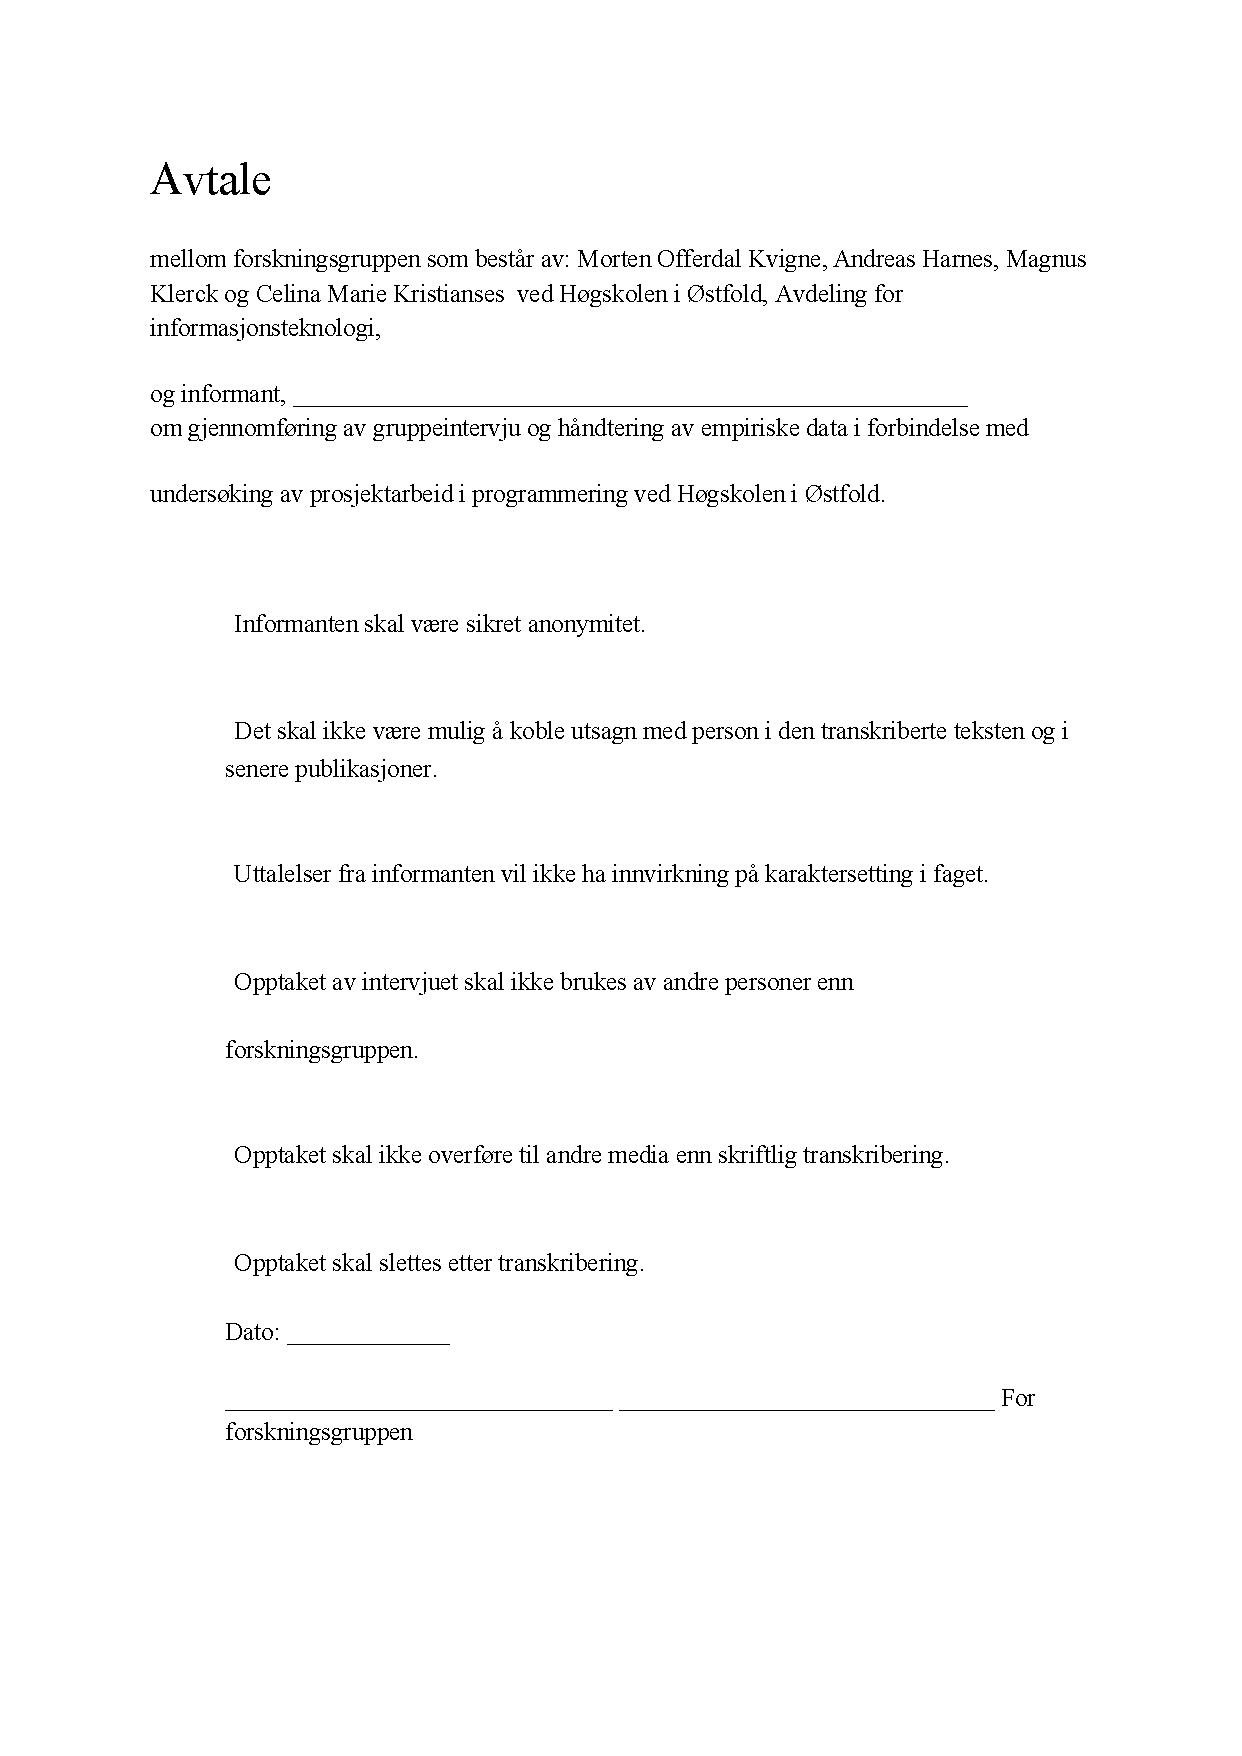
\includepdf[]{appendix/Avtale.pdf}
